%%%%%%%%%%%%%%%%%%%%%%%%%%%%%%%%%%%%%%%%%
% Short Sectioned Assignment
% LaTeX Template
% Version 1.0 (5/5/12)
%
% This template has been downloaded from:
% http://www.LaTeXTemplates.com
%
% Original author:
% Frits Wenneker (http://www.howtotex.com)
%
% License:
% CC BY-NC-SA 3.0 (http://creativecommons.org/licenses/by-nc-sa/3.0/)
%
%%%%%%%%%%%%%%%%%%%%%%%%%%%%%%%%%%%%%%%%%

%----------------------------------------------------------------------------------------
%	PACKAGES AND OTHER DOCUMENT CONFIGURATIONS
%----------------------------------------------------------------------------------------

\documentclass[paper=a4, fontsize=11pt]{scrartcl} % A4 paper and 11pt font size

\usepackage[T1]{fontenc} % Use 8-bit encoding that has 256 glyphs
%\usepackage{fourier} % Use the Adobe Utopia font for the document - comment this line to return to the LaTeX default
\usepackage[english]{babel} % English language/hyphenation
\usepackage{amsmath,amsfonts,amsthm} % Math packages
\usepackage{mathtools} %More math! (For dscases)
\usepackage{hyperref} %HTML package
\usepackage{pgfplots} %Makes plots in LaTeX
\usepackage{tikz} %Also tikz?
\usepgfplotslibrary{fillbetween}%Let's me fill between named plots
\usepackage{graphicx} %import pics
\graphicspath{ {Python_figs/} }
\DeclareGraphicsExtensions{.pdf,.png,.jpg}
\usepackage{sectsty} % Allows customizing section commands
\allsectionsfont{ \normalfont\scshape} % Make all sections the default font and small caps


\renewcommand{\thesubsection}{\alph{subsection}} %Make subsections start with letters

\usepackage{fancyhdr} % Custom headers and footers
\pagestyle{fancyplain} % Makes all pages in the document conform to the custom headers and footers
\fancyhead{} % No page header - if you want one, create it in the same way as the footers below
\fancyfoot[L]{} % Empty left footer
\fancyfoot[C]{} % Empty center footer
\fancyfoot[R]{\thepage} % Page numbering for right footer
\renewcommand{\headrulewidth}{0pt} % Remove header underlines
\renewcommand{\footrulewidth}{0pt} % Remove footer underlines
\setlength{\headheight}{13.6pt} % Customize the height of the header

\numberwithin{equation}{section} % Number equations within sections (i.e. 1.1, 1.2, 2.1, 2.2 instead of 1, 2, 3, 4)
\numberwithin{figure}{section} % Number figures within sections (i.e. 1.1, 1.2, 2.1, 2.2 instead of 1, 2, 3, 4)
\numberwithin{table}{section} % Number tables within sections (i.e. 1.1, 1.2, 2.1, 2.2 instead of 1, 2, 3, 4)

\setlength\parindent{0pt} % Removes all indentation from paragraphs - comment this line for an assignment with lots of text

%----------------------------------------------------------------------------------------
%	TITLE SECTION
%----------------------------------------------------------------------------------------

\newcommand{\horrule}[1]{\rule{\linewidth}{#1}} % Create horizontal rule command with 1 argument of height

\title{	Assignment 5}

\author{Benjamin Jakubowski} % Your name

\date{\normalsize\today} % Today's date or a custom date

\begin{document}

\maketitle % Print the title

%----------------------------------------------------------------------------------------
%	PROBLEM 1
%----------------------------------------------------------------------------------------

\section{Roulette}

\subsection{Probability of making money betting on a number}

If Bob bets on a number, then let
\[
X_i =
\begin{cases}
  1 & \textrm{if he wins (probability 1/38)}\\
  0 & \textrm{if he loses (probability 37/38)}\\
\end{cases}
\]

Then, his net earnings for 100 bets is
\[\sum_{i = 1}^{100} \left(36X_i - 1\right) = 36 \sum_{i = 1}^{100} X_i -100\]

Now, note his net earnings is positive if $\sum_{i = 1}^{100} X_i \geq 3$. Thus, we want to determine

\[P\left(\sum_{i = 1}^{100}X_i \geq 3 \right) = 1 - P\left(\sum_{i = 1}^{100}X_i \leq 2 \right)\]

Using the CLT, we know we can approximate the distribution of $\sum_{i = 1}^{100}X_i$ using the normal distribution

\[Z = \frac{\sum_{i = 1}^{100}X_i - 100 \cdot \frac{1}{38}}{\sqrt{100\cdot\frac{1}{38}\cdot\frac{37}{38}}} \approx \mathcal{N}(0,1)\]

Thus (noting we use 2.5, not 2, as a continuity correction in the following approximation):
\[P\left(\sum_{i = 1}^{100}X_i \leq 2 \right) \approx \Phi\left( \frac{2.5 - 100 \cdot \frac{1}{38}}{\sqrt{100\cdot\frac{1}{38}\cdot\frac{37}{38}}}\right) \approx .467244\]

So \[P\left(\sum_{i = 1}^{100}X_i \geq 3 \right) \approx 1 - .467244 = .532756\]

Note the exact probability (found using the CMF for the Binomial) is 0.491567. Our approximation has relatively high error due to the significant bias (i.e. $p = 1/38 << 0.5$) and relatively small sample size.

\subsection{Probability of making money betting on a color}

If Bob bets on a color, then let
\[
X_i =
\begin{cases}
  1 & \textrm{if he wins (probability 18/38)}\\
  0 & \textrm{if he loses (probability 20/38)}\\
\end{cases}
\]

Then, his net earnings for 100 bets is
\[\sum_{i = 1}^{100} \left(2X_i - 1\right) = 2 \sum_{i = 1}^{100} X_i -100\]

Now, note his net earnings is positive if $\sum_{i = 1}^{100} X_i \geq 51$. Thus, we want to determine

\[P\left(\sum_{i = 1}^{100}X_i \geq 51 \right) = 1 - P\left(\sum_{i = 1}^{100}X_i \leq 50 \right)\]

Again using the normal approximation for the binomial,

\[Z = \frac{\sum_{i = 1}^{100}X_i - 100 \cdot \frac{18}{38}}{\sqrt{100\cdot\frac{18}{38}\cdot\frac{20}{38}}} \approx \mathcal{N}(0,1)\]

Thus (noting we use 50.5, not 51, as a continuity correction in the following approximation):
\[P\left(\sum_{i = 1}^{100}X_i \leq 50 \right) \approx \Phi\left( \frac{50.5 - 100 \cdot \frac{18}{38}}{\sqrt{100\cdot\frac{18}{38}\cdot\frac{20}{38}}}\right) \approx .734731\]

So \[P\left(\sum_{i = 1}^{100}X_i \geq 51 \right) \approx 1 - .734731 = .26527\]

Note the exact probability (found using the CMF for the Binomial) is 0.2650235. Our approximation has comparatively lower error than the estimate for betting on a number since this binomial is much less biased (i.e. $p = 1/38 << 18/38 \approx 0.5$).

\subsection{Asymptotic performance of both betting strategies}

First, note when betting on a number,
\[E(36X_i -1) = 36E(X_i) -1 = 36 \cdot \frac{1}{38} - 1 = -\frac{1}{19}\]

and, when betting on a color,
\[E(2X_i -1) = 2E(X_i) -1 = 2 \cdot \frac{18}{38} - 1 = -\frac{1}{19}\]

Since the expected earnings per bet are the same, the law of large numbers implies these strategies are equivalent (since both will converge to $E = -\frac{1}{19}$ as $n \to \infty$.) However, if Bob votes on color his expected earnings will converge to $E = -\frac{1}{19}$ more quickly. To illustrate this, a histogram showing 1000 trials of 100 bets for each strategy is shown below. Note the distribution for betting on color is more concentrated around this expected value than for betting on a number.

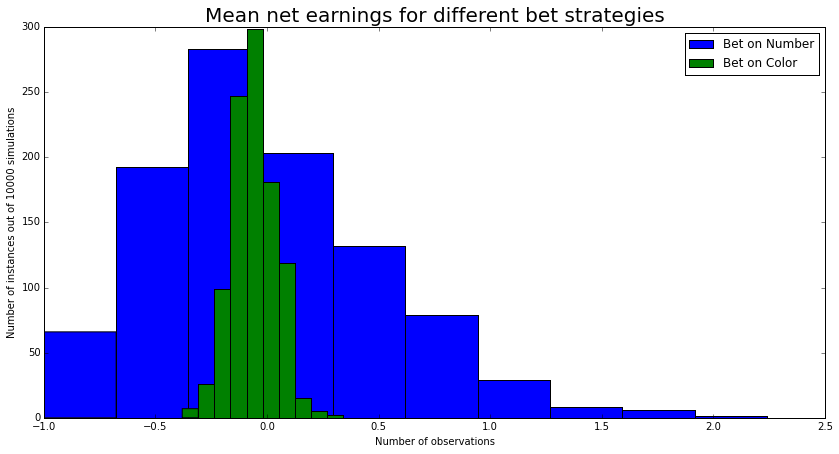
\includegraphics[scale=0.5]{Q1c_fig}

 \subsection{Expected gain, if Bob bet's on a number and makes money}
 
 First, note we will assume Bob is betting on a number (since it's the optimal strategy if his goal is to maximum the the probability of making money over 100 bets). Thus, if he made money, we know he must have won at least 3 bets. Thus, his expected gain is
\[E\left[36\cdot \sum_{i = 1}^{100} X_i -100 \big| \sum_{i = 1}^{100} X_i \geq 3\right] = 36 \cdot E\left[ \sum_{i = 1}^{100} X_i  \big| \sum_{i = 1}^{100} X_i \geq 3\right] - 100 \]

Now, applying the CLT, we can approximate the distribution $\sum_{i = 1}^{100} X_i$ as
\[X \sim \mathcal{N}(100\cdot 1/38, 100\cdot1/38\cdot37/38)\]
Next, to solve this problem, we could derive the conditional PDF $f_{X|X>2.5}(x)$ then integrate
\[\int_{2.5}^{\infty} x \cdot f_{X|X>2.5}(x) \textrm{d}x\]
However, this distribution is already well described (it's called the truncated normal distribution), and it's expected value is given on wikipedia as
\[E(X | X>a) = \mu + \sigma \cdot \frac{\phi(\frac{a - \mu}{\sigma})}{1 - \Phi(\frac{a - \mu}{\sigma})}\]
Using this formula (noting $\phi$ and $\Phi$ are the standard normal PDF and CDF, respectively), we find:
\[E(X | X>2.5) = 100\cdot1/38 + \sqrt{100\cdot1/38\cdot37/38} \cdot \frac{\phi\left(\frac{2.5 - 100\cdot1/38}{\sqrt{100\cdot1/38\cdot37/38}}\right)}{1 - \Phi\left(\frac{2.5 - 100\cdot1/38}{\sqrt{100\cdot1/38\cdot37/38}}\right)}\]

Note
\[\phi\left(\frac{2.5 - 100\cdot1/38}{\sqrt{100\cdot1/38\cdot37/38}}\right) = 0.3975968\]
\[1-\Phi\left(\frac{2.5 - 100\cdot1/38}{\sqrt{100\cdot1/38\cdot37/38}}\right) = 0.532756\]

Therefore, 
\[E(X | X>2.5) = 3.8262\]
so the expected gain is $36 \cdot 3.8262 - 100 =  37.7432$.\\

Thus, using the CLT and the normal approximately we expect Bob gained \$37.74. This is close to the exact answer (found much more simply, directly, and accurately using the appropriate conditional binomial distribution), which is \$42.18.

%----------------------------------------------------------------------------------------
%	PROBLEM 2
%----------------------------------------------------------------------------------------

\section{Weight}

\subsection{Minimum sample size}

Recall we are trying to determine the minimum sample size necessary to construct a rigorous 95\% confidence interval of width 5lb on the population mean weight.

By corollary 1.21 (in the notes), if b is an upper bound on the variance $Var(X_i)$,

\[P\left(\mu \in \left[\bar{X}_n - \frac{b}{\sqrt{\alpha n}}, \bar{X}_n - \frac{b}{\sqrt{\alpha n}}\right]\right) \geq 1 - \alpha\]

Now, if the heaviest man ever recorded weighed 1400 lbs, then we can use this as our bound $b$ on the variance. Thus, with $b = 1400$ and $\alpha = 0.05$, we want
\[\frac{b}{\sqrt{\alpha n}} = \frac{1400}{\sqrt{0.05 n}} \leq 2.5\]
\[\implies \frac{1400^2}{2.5^2 \cdot 0.05} \leq n\]
\[\implies 6272000 \leq n\]

Obviously this is an absurdly large sample size. Thus, we need to make additional assumptions (or use additional information) to get a more reasonable lower bound on $n$.

\subsection{Minimum sample size using sample variance}
Now, recall that for large n

\[P\left(\mu \in \left[\bar{X}_n - \frac{s}{\sqrt{n}}\Phi(\alpha/2), \bar{X}_n - \frac{s}{\sqrt{n}}\Phi(\alpha/2)\right]\right) \approx 1 - \alpha\]

So, for $\alpha = 0.05$, $s^2 = 1000$, we want
\[\frac{\sqrt{1000}}{\sqrt{n}} \Phi(\frac{0.05}{2}) = \frac{\sqrt{1000}}{\sqrt{n}} 1.96 \leq 2.\]
\[\implies \left(\frac{\sqrt{1000}1.96}{2.5}\right)^2 \leq n \]
\[\implies 614.656 \leq 615 \leq n \]

So, to achieve our desired power, we need a minimum of 615 people.

\subsection{Generating and analyzing confidence intervals}

The first interesting observation from the simulations run in the $confidence\_intervals.py$ script is the number of confidence intervals that contain the true mean when $n=20$ versus $n=1000$. When I ran the simulation, when $n=20$ 681 of 10000 intervals didn't contain the true mean , while only 511 intervals out of 10000 didn't contain the true mean when $n=1000$. This result makes sense- the confidence intervals being constructed are approximate confidence intervals constructed using the normal approximation. This approximation is derived from the CLT, which describes convergence as $n$ grows large. Thus, we would expect our interval to perform poorly for small $n$, such as $n=20$.

The other interesting observation is the sample variance distribution when $n = 20$ and $n=1000$. The plot is provided below for reference:

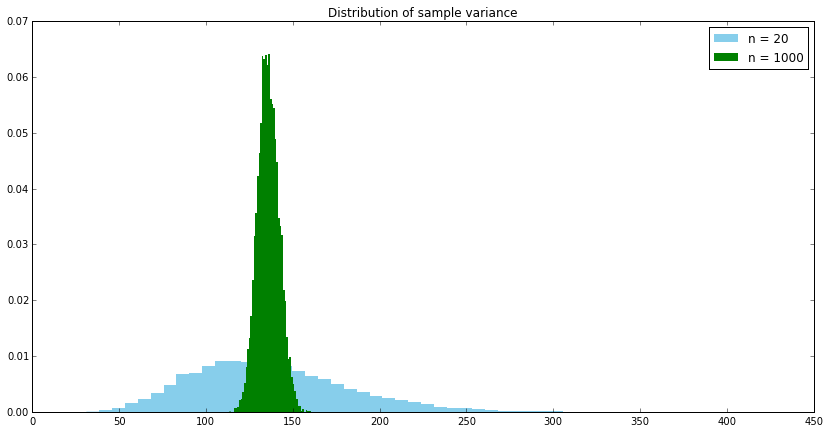
\includegraphics[scale=0.5]{Q2c_fig}

As you can see in the plot, as $n$ grows larger, the sample variance also converges in distribution. Also, when $n$ is small, the variance in sample variance (i.e. $Var(s^2)$) is much greater, and the distribution is right skewed (which makes sense, given sample variance is bounded by 0 on the left).


%----------------------------------------------------------------------------------------
%	PROBLEM 3
%----------------------------------------------------------------------------------------

\section{Convergence in probability implies convergence in distribution}

\subsection{Bounding $P(A_n \leq a)$}

We will show
\[P(A\leq a - \epsilon) - P(|A_n - A| > \epsilon) \leq P(A_n \leq a) \leq P(A \leq a + \epsilon) + P(|A_n - A| > \epsilon)\]

First, let:
\begin{itemize}
\item $B$ be the event $A \leq a - \epsilon$
\item $C$ be the event $|A_n - A| \leq \epsilon$
\item $D$ be the event $A_n \leq a$
\end{itemize}

Now note $(B \cap C) \subseteq D$ (since $B \cap C$ implies $P(D) = 1$). Thus, $P(B \cap C) \leq P(D)$. But
\begin{align*}
P(B \cap C) &= P(B) + P(C) - P(B \cup C) \\
   &= P(B) + (1 - P(C^c)) - P(B \cup C)\\
   &= P(B) - P(C^c) + (1 - P(B \cup C)) \\
\end{align*}

But then, since $(1 - P(B \cup C)) \geq 0$, we know $P(B \cap C) \geq P(B) - P(C^c)$. Thus, $P(B) - P(C^c) \leq P(D)$, so
\[P(A\leq a - \epsilon) - P(|A_n - A| > \epsilon) \leq P(A_n \leq a)\]

To see the upper bound, note
\[P(A_n \leq a) = P(A_n \leq a, A \leq a + \epsilon) + P(A_n \leq a, a + \epsilon < A)\]

Now let: 
\begin{itemize}
\item $F$ be the event $A_n \leq a, a + \epsilon < A$
\item $G$ be the event $|A_n - A| > \epsilon$
\end{itemize}

Then $F \subseteq G$, so $P(F) \leq P(G)$. Similarly, note by event (set) containment we have
\[P(A_n \leq a, A \leq a + \epsilon) \leq P(A \leq a + \epsilon)\]

Thus,
\[P(A_n \leq a) = P(A_N \leq a, A \leq a + \epsilon) + P(A_N \leq a, A \leq a + \epsilon) \leq  P(A \leq a + \epsilon) +  P(|A_N - A| > \epsilon) \]

Finally, combining these bounds, we have 
\[P(A\leq a - \epsilon) - P(|A_n - A| > \epsilon) \leq P(A_n \leq a) \leq P(A \leq a + \epsilon) + P(|A_n - A| > \epsilon)\]

\subsection{Prove $A_n \to A$ in distribution}

Assume $A_n \to A$ in probability, then (fixing $\epsilon$),
\[\lim_{n \to \infty} P(|A - A_n| > \epsilon) = 0\]
Now, let's take the limit as $n \to \infty$ of the expression derived in (a).
\[\lim_{n \to \infty} \left[P(A\leq a - \epsilon) - P(|A_n - A| > \epsilon) \leq P(A_n \leq a) \leq P(A \leq a + \epsilon) + P(|A_n - A| > \epsilon)\right]\]

By convergence in probability, this becomes
\[P(A\leq a - \epsilon)> \epsilon) \leq \lim_{n \to \infty}P(A_n \leq a) \leq P(A \leq a + \epsilon)\]

Now let's assume $a$ is a continuity point of $F_A$. We can rewrite this expression using the CDFs $F_{A_n}$ and $F_A$.
\[F_A(a - \epsilon) \leq  \lim_{n \to \infty}F_{A_n}(a) \leq F_A(a + \epsilon) \]
 
Since $a$ is a continuity point of $F_A$, when we take the limit as $\epsilon \to \infty$

\[\lim_{\epsilon \to \infty} \left[F_A(a - \epsilon) \leq  \lim_{n \to \infty}F_{A_n}(a) \leq F_A(a + \epsilon)\right] \]
\[F_A(a) \leq  \lim_{n \to \infty}F_{A_n}(a) \leq F_A(a) \]

Thus, for all continuity points of $F_{A}$, we have $\lim_{n \to \infty}F_{A_n}(a) = F_A(a)$, so $A_n$ converges to $A$ in distribution.

\subsection{Counter-example for the converse}

Now note convergence in distribution doesn't imply convergence in probability. To see this, imagine flipping a fair coin. For all $n \in \mathbb{N}$, let
\[
X_n =
\begin{cases}
 0 & \textrm{if tails}\\
 1 & \textrm{if heads}\\
\end{cases}
\]

Then let 
\[
X=
\begin{cases}
 0 & \textrm{  if heads} \\
 1 & \textrm{  if tails}\\
\end{cases}
\]
Then $\lim_{n \to \infty} P_{X_n}(x) = P_X(x)$ (trivially). However, $X_n$ clearly does not converge in probability to $X$. To see this, simply note $|X_n - X| = 1$ for all $n \in \mathbb{N}$.

%----------------------------------------------------------------------------------------
%	PROBLEM 4
%----------------------------------------------------------------------------------------

\section{Radioactive Sample}

\subsection{Using running mean to estimate $c$ for sample 1}

First, the running sample mean for data in $radioactive\_sample\_1.txt$ is shown below:

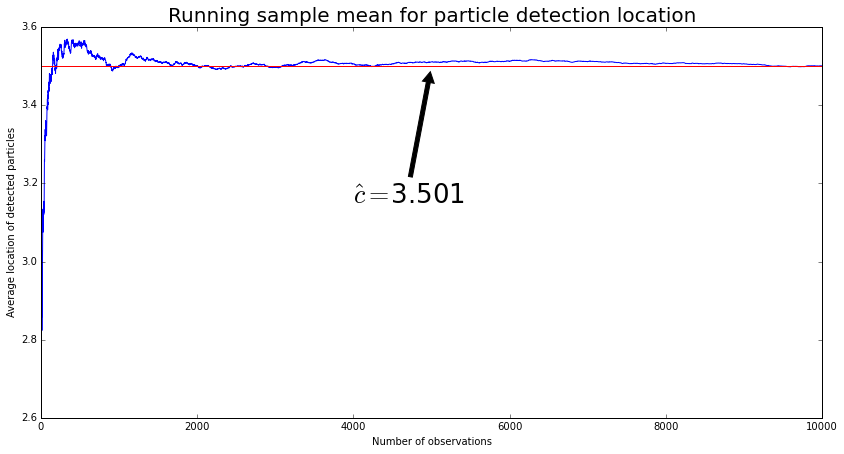
\includegraphics[scale=0.5]{Q4a_fig}

Our estimate of $c$ is $\hat{c} = 3.501$. To get this value, I noticed the running means appear to converge. Therefore, given 10,000 observations, our best estimator is the mean of all the observations (or the final running mean), which in this case equals 3.501.

\subsection{Using running mean to estimate $c$ for sample 2}

The running sample mean for data in $radioactive\_sample\_2.txt$ is shown below:

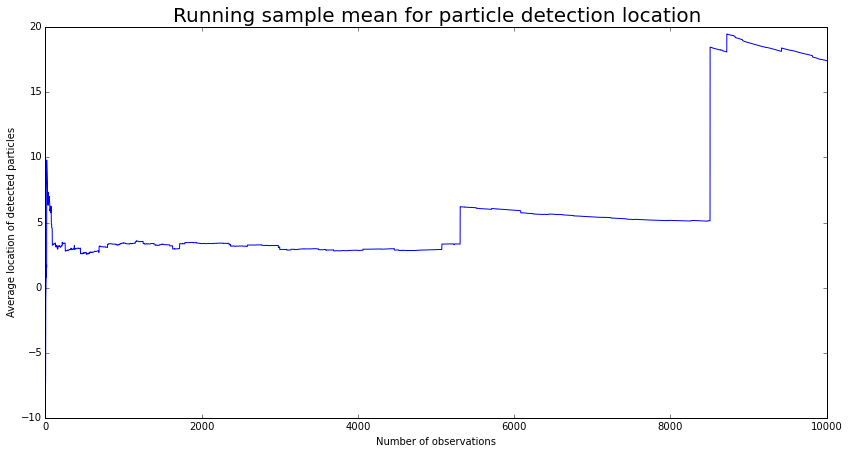
\includegraphics[scale=0.5]{Q4b_fig}

Looking at this plot, it is clear the sample means don't converge. Thus, our method for estimating $c$ does not work in this case.

\subsection{Deriving a pdf and mean of $X$}

Recall the sample is a unit distant from the line of sensors. If $A \sim U[-\pi /2, \pi /2]$ models $\alpha$ (the angle between the vertical axis and the particles trajectory), then $X = \textrm{tan}(A)$, so $A = \textrm{tan}^{-1}(x)$. Thus (first recalling $\textrm{tan}^{-1}(x)$ inceases monotonically)
\begin{align*}
F_X(x) &= P(X \leq x) \\
   &= P(\textrm{tan}^{-1}(X) \leq \textrm{tan}^{-1}(x)) \\ 
   &= P(A \leq \textrm{tan}^{-1}(x)) \\ 
   &= F_A(\textrm{tan}^{-1}(x)) \\ 
   &= \frac{\textrm{tan}^{-1}(x) - (-\pi/2)}{\pi/2 - (-\pi/2)} \\ 
   &= \frac{\textrm{tan}^{-1}(x) + \pi/2}{\pi} \\ 
   &= 1/\pi \cdot \textrm{tan}^{-1}(x) + 1/2
\end{align*} 

Then
\[f_X(x) = F_X'(x) = \frac{1}{\pi \cdot (1 + x^2)}\]

Now note this is the standard Cauchy distribution, and its mean is undefined. This model would explain my observations in (b). As previously noted, the running sample means don't appear to converge. This is expected behavior for a Cauchy distribution. Additionally, the frequent extreme observations (observed in the running mean plot as large jumps) reflect the fat tails of the Cauchy (i.e. the relatively high probability of extreme values).


\subsection{Sampling four different IID vectors from the Cauchy}

Below is a plot of the running sample means for four different IID vectors (length 10000) sampled from the Cauchy distribution.

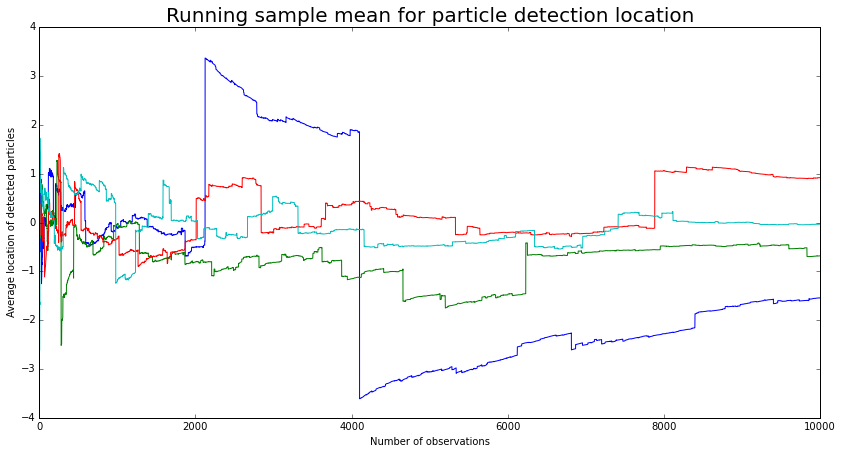
\includegraphics[scale=0.5]{Q4d_fig}

Again, as expected, we don't observe the running means converging to any central value. We do observe the running means frequently jumping in response to an extreme observation (which, as stated above, is characteristic of the Cauchy distribution).

%----------------------------------------------------------------------------------------
%	PROBLEM 5
%----------------------------------------------------------------------------------------

\section{Election poll}

\subsection{Using the sample mean to estimate the outcome of the election}

Assume the $R_i$ are IID. This assumption is reasonable if the individuals polled are approximately random draws from a sufficiently large population, such that sampling without replacement and sampling with replacement are approximately equivalent.

Given this assumption, then the law of large numbers implies
\[\bar{R}_n = 1/n \sum_{i = 1}^n R_i\]
is a consistent estimator of $\theta_r$, the true percentage of the population that will vote republican.

\subsection{Predicting the outcome of the election}

Given the data, our estimate of the population proportion voting republican is

\[\hat{\theta}_r = \bar{R}_n = 1/94000 \sum_{i = 1}^{94000} R_i = \frac{45000}{45000+49000} \approx 0.4787\]

Thus we predict the Democrats will win the election.

To quantify the accuracy of our estimate, we want to place an upper bound on
\[P\left( \theta_r \notin (\bar{R}_n - | \bar{R}_n - 0.5|,  \bar{R}_n +  | \bar{R}_n - 0.5| )\right) = P(|\theta_r - \bar{R}_n| > |\bar{R}_n - 0.5| )\]

Recalling $E(\bar{R}_n) = \theta_r$, we can apply Chebyshev's inequality, yielding:
\[P(|\theta_r - \bar{R}_n| > |\bar{R}_n - 0.5| ) \leq \frac{Var(\bar{R}_n)}{(\bar{R}_n-0.5)^2}\]

Now, since $Var(R_i) \leq 1$
\[Var(\bar{R}_n) = \frac{1}{94000^2} \sum_{i = 1}^{94000} Var(R_i) \leq \frac{1}{94000^2} \cdot 1\cdot 94000 =  \frac{1}{94000}\]

Thus,
\begin{align*}
P(|\theta_r - \bar{R}_n| > |\bar{R}_n - 0.5| ) &\leq \frac{1/94000}{(\bar{R}_n-0.5)^2} \\
   &=  \frac{1/94000}{(45000/94000-0.5)^2}\\
   &= \frac{1/94000}{(2000/94000)^2} \\
   &=  \frac{94000}{(2000)^2} = 0.0235
\end{align*}

Thus (given our assumptions of IID random draws from the population) the probability our prediction is incorrect is less than 0.0235.

\subsection{Using the sample mean to estimate the outcome of the election}

First, let
\[\sum_{i = 1}^n Y_i = R_y\]
be the number of young people responding republican. and
\[\sum_{i = 1}^n O_i = R_o\]
be the number of old people responding republican.
Then $X_{n_1, n_2} = a\cdot R_y + b \cdot R_o$.

Now, if $X_{n_1, n_2}$ is unbiased, then
\[ E(X_{n_1, n_2}) = \theta_r = p_y \cdot r_y + p_o \cdot r_o\]
where
\begin{itemize}
\item $\theta_r$ is the proportion of republicans in the overall population
\item $p_y$/$p_o$ are the proportions of the population that are young/old
\item $r_y$/$r_o$ are the proportions of the young/old subpopulations that are republican
\end{itemize}

Now note
\[ E(X_{n_1, n_2}) = E(a\cdot R_y + b \cdot R_o) = a\cdot E(R_y) + b \cdot E(R_o) \]
Next, recall the definitions of $R_y$ and $R_o$. Assuming the $Y_i$ and $O_i$ are IID, the law of large numbers implies $E(R_y) = n_1 \cdot r_y$ and $E(R_o) = n_2 \cdot r_o$.
Thus, $E(X_{n_1, n_2})$ will be unbiased if
\[a\cdot E(R_y) + b \cdot E(R_o) = a\cdot  n_1 \cdot r_y + b \cdot n_2 \cdot r_o = p_y \cdot r_y + p_o \cdot r_o\]
Which implies
\[ a = p_y \cdot \frac{1}{n_1} \]
\[ b = p_o \cdot \frac{1}{n_2} \]


\subsection{Using the new estimator to predict the election}

First, we must norm the population proportions over the voting age population. Then
\[p_y = \frac{0.20}{0.75}\]
\[p_o = \frac{0.55}{0.75}\]

Then our estimator is
\[\hat{\theta}_r = X_{n_1, n_2} =  p_y \cdot \frac{1}{n_1} \cdot R_y + p_o \cdot \frac{1}{n_2} \cdot R_o = \frac{0.20}{0.75} \cdot \frac{1}{59000} \cdot 24000 + \frac{0.55}{0.75} \cdot \frac{1}{35000} \cdot 21000 \approx 0.56655\] 

Thus, using our new estimator, we would now predict the republicans win. Note this assumes the proportions of young/old people in the population of voters is the same as in the population at large.

Finally, to quantify the precision of our estimate, recall we must bound the probability 
\[P\left( \theta_r \notin (X_{n_1, n_2} - |X_{n_1, n_2} - 0.5|,  X_{n_1, n_2} +  |X_{n_1, n_2} - 0.5| )\right) = P(|\theta_r - X_{n_1, n_2}| > |X_{n_1, n_2} - 0.5| )\]
Recalling $E(X_{n_1, n_2}) = \theta_r$, we can apply Chebyshev's inequality, yielding:
\[P(|\theta_r - X_{n_1, n_2}| > |X_{n_1, n_2} - 0.5| ) \leq \frac{Var(X_{n_1, n_2})}{(X_{n_1, n_2}-0.5)^2}\]

Now note
\begin{align*}
Var(X_{n_1, n_2}) &= Var(p_y \cdot \frac{1}{n_1} \cdot R_y + p_o \cdot \frac{1}{n_2} \cdot R_o)\\
   &= \left(\frac{p_y}{n_1}\right)^2 \cdot \sum_{i = 1}^{n_1}Var(Y_i) + \left(\frac{p_o}{n_2}\right)^2 \cdot \sum_{i = 1}^{n_2}Var(O_i) \\
   &\leq \left(\frac{p_y^2}{n_1}\right) + \left(\frac{p_o^2}{n_2}\right) \qquad{}\textrm{ (since }Var(Y_i)\leq1, Var(O_i) \leq 1)
\end{align*}

Substituting, we get
\[ P(|\theta_r - X_{n_1, n_2}| > |X_{n_1, n_2} - 0.5| ) \leq \frac{\left(\frac{p_y^2}{n_1}\right) + \left(\frac{p_o^2}{n_2}\right)}{(X_{n_1, n_2}-0.5)^2} = \frac{\left(\frac{(0.20/0.75)^2}{59000}\right) + \left(\frac{0.55/0.75^2}{35000}\right)}{(0.56655-0.5)^2} \approx 0.003144 \]

Thus, 
\[P\left( \theta_r \notin (X_{n_1, n_2} - |X_{n_1, n_2} - 0.5|,  X_{n_1, n_2} +  |X_{n_1, n_2} - 0.5| )\right) \approx 0.003144\]

So (given our assumptions of IID random draws from the two subpopulation) the probability our prediction is incorrect is less than 0.003144.
 %----------------------------------------------------------------------------------------
\end{document}